% =====================================================================
% Priority-Based Network Traffic Management for Campus Networks
% IEEE Conference Paper — Full Draft
% CS23502 Mini-Project, MIT Campus, Anna University
% =====================================================================
\documentclass[conference]{IEEEtran}
\IEEEoverridecommandlockouts

\usepackage{cite}
\usepackage{amsmath,amssymb,amsfonts}
\usepackage{algorithmic}
\usepackage{algorithm}
\usepackage{graphicx}
\usepackage{textcomp}
\usepackage{xcolor}
\usepackage{booktabs}
\usepackage{url}
\usepackage{hyperref}

\def\BibTeX{{\rm B\kern-.05em{\sc i\kern-.025em b}\kern-.08em
    T\kern-.1667em\lower.7ex\hbox{E}\kern-.125emX}}

\begin{document}

% =====================================================================
\title{Priority-Based Network Traffic Management for Campus Networks
Using Software-Defined Networking and Behavioral Classification}

\author{
\IEEEauthorblockN{Yazhene S}
\IEEEauthorblockA{Reg. No.: 2024503552\\
\textit{Dept. of Computer Science and Engineering}\\
MIT Campus, Anna University\\
Chennai, India\\
yazh.yazhene@gmail.com}
\and
\IEEEauthorblockN{Yamica V}
\IEEEauthorblockA{Reg. No.: 2024503302\\
\textit{Dept. of Computer Science and Engineering}\\
MIT Campus, Anna University\\
Chennai, India\\
yamicavarrunkumar@gmail.com}
\and
\IEEEauthorblockN{Tanishka K}
\IEEEauthorblockA{Reg. No.: 2024503530\\
\textit{Dept. of Computer Science and Engineering}\\
MIT Campus, Anna University\\
Chennai, India\\
tanishkakathervel496@gmail.com}
\and
\IEEEauthorblockN{Monica R}
\IEEEauthorblockA{Reg. No.: 2024503510\\
\textit{Dept. of Computer Science and Engineering}\\
MIT Campus, Anna University\\
Chennai, India\\
moni142006@gmail.com}
}

\maketitle

% =====================================================================
\begin{abstract}
On a shared campus network link, video-conferencing traffic and
large-file downloads are treated identically by default. Under
contention the video call degrades—dropped frames and lag—even
though it is far more delay-sensitive than the download. We propose
and evaluate a Software-Defined Networking (SDN) system that
automatically classifies network flows by their observed packet-level
behavior and enforces differentiated Quality-of-Service (QoS) without
manual configuration or static IP/port rules. A shallow decision-tree
classifier extracts six behavioral features per 20-packet window and
assigns each flow to one of three service tiers (real-time, best-effort,
bulk). An os-ken/OpenFlow~1.3 controller then maps classified flows to
Linux-HTB queues with guaranteed minimum bandwidth floors (6/2/1~Mbps)
and borrowable ceilings (10/8/10~Mbps), following a starvation-safe
design that prevents lower-priority traffic from being completely starved.
A React/Node.js dashboard provides live per-tier monitoring and an
on/off control. Evaluation in a Mininet-emulated topology demonstrates
an 84\% reduction in real-time jitter (5.11~ms to 0.84~ms) and a
classifier holdout accuracy of 97.6\% on 288 fresh balanced samples,
with zero realtime packet loss. Source code is available at
\url{https://github.com/YazheneS/priority-based-network-trafficing}.
\end{abstract}

\begin{IEEEkeywords}
Software-Defined Networking, Quality of Service, Traffic Classification,
OpenFlow, Mininet, Decision Tree, Campus Networks, HTB Queuing
\end{IEEEkeywords}

% =====================================================================
\section{Introduction}
\label{sec:intro}

Campus networks routinely carry heterogeneous traffic—video
conferencing, interactive browsing, and bulk file transfers—sharing
the same physical link. Without differentiation, these flows compete
equally for bandwidth. When a large file transfer saturates the link,
real-time flows such as video calls suffer disproportionately because
even small queuing delays accumulate into perceptible jitter and
latency.

Traditional QoS approaches address this through static rules: fixed
IP addresses or TCP/UDP port numbers determine priority, with bandwidth
assigned to each class by hand. Deo et al.~\cite{deo2024} instead
allocate bandwidth to OpenFlow QoS classes purely from observed flow
statistics via OpenFlow meters, avoiding manually fixed per-class
shares; this motivates deriving allocation and classification decisions
from observed traffic behavior rather than static configuration.
Software-Defined Networking (SDN) offers a programmable alternative
where flow management is centralized, but static SDN rules suffer the
same brittleness. Gorkemli et al.~\cite{gorkemli2015} show that strict
priority-based scheduling—always serving tier~1 before tier~2 before
tier~3—risks completely starving lower-priority traffic under sustained
higher-priority load. Related QoS mechanisms in the wider literature
span meter- and slicing-based burst control~\cite{slicing2025}, hybrid
IP/SDN QoS architectures~\cite{hussein2025}, scalable low-latency
transport~\cite{fairhurst2021}, campus-network QoS
policy~\cite{qospolicies2019}, application-specific video QoS over
SDN~\cite{almaqri2016,shvc2022}, and cautions on emulation-based SDN
evaluation~\cite{emulation2022}, all consulted while scoping this
project's design space.

This work addresses both limitations by combining behavioral traffic
classification with a fairness-aware SDN priority engine. Serag et
al.~\cite{serag2025} demonstrate that packet-size and timing statistics
alone are sufficient to distinguish interactive from bulk traffic
without deep packet inspection. Shahriar et al.~\cite{shahriar2024}
formalize a bandwidth-splitting scheme with guaranteed minimum floors
per tier, preventing starvation while still enforcing priority.

Our contribution is the integration of these four ideas into a single,
fully automated pipeline: no single prior system combines behavioral
classification, starvation-safe queuing, live enforcement via
OpenFlow, and a monitoring dashboard end-to-end. We implement, test,
and measure this system in a Mininet topology under controlled
traffic, reporting before/after results across all three service tiers.

% =====================================================================
\section{Related Work}
\label{sec:related}

\subsection{Flow-Statistics-Based Allocation}
Deo et al.~\cite{deo2024} propose an adaptive bandwidth allocation
algorithm that uses OpenFlow meters and per-flow statistics collected
directly from switches, rather than fixed, manually assigned shares
per class. Their flow-statistics-driven approach motivates our use of
observed behavior, rather than static configuration, to drive
allocation decisions.

\subsection{Strict Scheduling Risks}
Gorkemli et al.~\cite{gorkemli2015} critique strict-precedence
OpenFlow prioritization, where higher tiers are always served first:
under sustained high-priority load, lower-priority queues can be
starved of service. Their critique motivates the guaranteed-floor
design we adopt: every tier retains a non-zero minimum, even under
contention.

\subsection{Behavioral Traffic Classification}
Serag et al.~\cite{serag2025} classify network flows using per-packet
statistical features (mean and variance of packet size and
inter-arrival time) through a machine-learning model, without
inspecting payload content. This approach is robust to encryption and
port reassignment. We extend it with a sixth feature—achieved byte
rate across a packet window—to resolve overlap between rate-limited
real-time streams and uncapped bulk streams that share similar
packet-level timing statistics.

\subsection{Fairness-Aware Bandwidth Splitting}
Shahriar et al.~\cite{shahriar2024} formalize weighted bandwidth
allocation with per-tier guaranteed minimums in SDN environments. The
tier receives at least its guaranteed rate regardless of higher-tier
demand, and can borrow spare capacity up to a ceiling when other tiers
are idle. We implement this formulation directly in our Linux-HTB queue
configuration.

% =====================================================================
\section{System Model}
\label{sec:model}

Let the shared link have capacity $C$ (10~Mbps in our evaluation).
Define three service tiers $\mathcal{T} = \{t_0, t_1, t_2\}$
(real-time, best-effort, bulk). Each tier $t_i$ is assigned:
\begin{itemize}
  \item A guaranteed minimum rate $g_i > 0$, such that
        $\sum_i g_i \leq C$.
  \item A ceiling $c_i \leq C$, the maximum rate tier $t_i$ may
        consume when spare capacity is available.
\end{itemize}

In our configuration, $g = [6, 2, 1]$~Mbps and $c = [10, 8, 10]$~Mbps.
The sum of guarantees is $9 \leq 10 = C$, leaving 1~Mbps of
over-subscription headroom.

Each incoming flow $f$ is characterized by a feature vector
$\mathbf{x}_f \in \mathbb{R}^6$ extracted from a sliding window
of $W = 20$ packets:
\begin{equation}
\mathbf{x}_f = \bigl[\mu_s,\,\sigma_s,\,\mu_\tau,\,\sigma_\tau,\,
               B_f,\,R_f\bigr]
\label{eq:features}
\end{equation}
where $\mu_s$ and $\sigma_s$ are the mean and standard deviation of
packet sizes, $\mu_\tau$ and $\sigma_\tau$ are the mean and standard
deviation of inter-arrival times, $B_f = \sigma_s / \mu_s$ is the
burstiness ratio, and $R_f = \sum_w \text{size}_w / \Delta T_w$ is
the achieved byte rate over window duration $\Delta T_w$.

A decision tree classifier $\hat{t} = h(\mathbf{x}_f)$ maps each
feature vector to a tier prediction. The controller then installs an
OpenFlow rule assigning flow $f$ to the corresponding HTB queue.

% =====================================================================
\section{Proposed System Architecture}
\label{sec:architecture}

The system comprises four interconnected components forming a
closed-loop pipeline, as shown in Fig.~\ref{fig:architecture}.

\begin{figure}[h]
\centering
\fbox{\parbox{0.9\columnwidth}{\centering\vspace{0.3cm}
\textbf{Traffic Sources} (h1, h2, h3)\\
$\downarrow$\\
\textbf{Open vSwitch s1} (Q0/Q1/Q2 HTB queues)\\
$\updownarrow$ \hspace{0.5cm} $\updownarrow$\\
\textbf{Classifier} \hspace{0.3cm} \textbf{Controller (os-ken)}\\
(6-feature DT) \hspace{0.3cm} (OpenFlow 1.3 rules)\\
$\downarrow$\\
\textbf{Dashboard} (React/Node.js)
\vspace{0.3cm}}}
\caption{Four-component system architecture: traffic sources feed the
SDN switch, which mirrors traffic to the classifier; the controller
installs per-flow rules; the dashboard monitors and controls the engine.}
\label{fig:architecture}
\end{figure}

\textbf{Mininet Topology:} Four virtual hosts (h1–h4) connected via
a single Open vSwitch (s1) emulate a campus access segment. h1, h2,
and h3 generate real-time (UDP, port~5000), best-effort (TCP, port~5100),
and bulk (TCP, port~5201) traffic respectively toward h4. The link
capacity is 10~Mbps.

\textbf{SDN Priority Engine:} The os-ken controller configures three
Linux-HTB queues on s1's egress port and installs OpenFlow~1.3 rules
mapping each classified flow to its queue. Port-match rules at
priority~20 direct real-time and bulk traffic to Q0 and Q2; a
priority-5 catch-all IP rule routes best-effort to Q1.

\textbf{Behavioral Classifier:} A shallow decision tree (max depth~4)
trained on 1,701 real Mininet-captured flows classifies each 20-packet
window into a tier. Classification runs in a live sniffing loop on the
switch interface.

\textbf{Live Dashboard:} A React frontend subscribes to a Node.js
WebSocket backend that polls per-tier metrics. An ON/OFF toggle sends
a REST call to the controller's \texttt{/toggle} endpoint, enabling
real-time before/after comparison.

% =====================================================================
\section{Algorithm}
\label{sec:algorithm}

% =====================================================================
% System Implementation (Weeks 5-8) -- paste into main.tex where the
% Month 2 / implementation section belongs. Uses the same \cite keys as
% the Review 1 paper (adjust to your actual BibTeX keys if they differ:
% gorkemli2015 -> IEEE 7130421, shahriar2024 -> arXiv:2403.15975,
% deo2024 -> PeerJ CS 2024, serag2025 -> Springer JNSM 2025).
%
% Preamble requirements (add once to main.tex if not already present):
%   \usepackage{algorithm}
%   \usepackage{algpseudocode}   % or \usepackage{algorithmic} for older style
% =====================================================================

\section{System Implementation}
\label{sec:implementation}

The baseline experiments established degradation of real-time traffic under
contention. This section describes the implementation of the four-layer
pipeline that
addresses it: an SDN priority engine, a behavioral traffic classifier, the
integration bridge connecting the two, and a live monitoring dashboard.

\subsection{SDN-Based Priority Engine}
\label{subsec:priority-engine}

The priority engine is implemented as an os-ken\footnote{os-ken is the
actively maintained fork of the now-unmaintained Ryu SDN framework.}
controller application operating over OpenFlow~1.3 on an Open vSwitch
instance within a Mininet-emulated topology. Rather than relying solely on
strict priority-based scheduling, we implement a three-tier, fairness-aware scheme
with a guaranteed minimum-bandwidth floor per tier, following the bandwidth-
splitting formulation of Shahriar et al.~\cite{shahriar2024}. The use of
multiple QoS queues and priority-based treatment is consistent with the SDN
QoS approach studied by Gorkemli et al.~\cite{gorkemli2015}.

Each tier is bound to a Linux-HTB queue on the switch's egress port:

\begin{table}[h]
\centering
\caption{Tier-to-queue configuration}
\label{tab:queue_configuration}
\begin{tabular}{lcccl}
\hline
\textbf{Tier} & \textbf{Queue} & \textbf{Guaranteed Rate}
& \textbf{Ceiling} & \textbf{OpenFlow Priority} \\
\hline
Real-time (video) & 0 & 6 Mbps & 10 Mbps & 20 \\
Best-effort (browsing) & 1 & 2 Mbps & 8 Mbps & 5 \\
Bulk (downloads) & 2 & 1 Mbps & 10 Mbps & 20 \\
\hline
\end{tabular}
\end{table}

The guaranteed rate represents the minimum bandwidth floor assigned to
each queue rather than a hard bandwidth cap. The ceiling represents the
maximum rate available to the queue, allowing unused capacity to be
utilized when other traffic classes do not consume their allocated
bandwidth. This implements the fairness-aware bandwidth-splitting
approach of Shahriar et al.~\cite{shahriar2024}, while providing a guaranteed
minimum bandwidth floor for every traffic tier.

The real-time queue receives a 6~Mbps guaranteed floor and a 10~Mbps
ceiling. Best-effort traffic receives a 2~Mbps guaranteed floor and an
8~Mbps ceiling, while bulk traffic receives a 1~Mbps guaranteed floor
and a 10~Mbps ceiling. The non-zero floor for bulk traffic is
intentional: although bulk traffic is deprioritized during contention,
it is not completely starved.

Thus, the configured ceiling is not a hard cap imposed independently of
available capacity; it provides borrowable headroom when other tiers
are not using their guaranteed share. Setting the guaranteed rate equal
to the ceiling would instead create a hard-cap configuration and would
not represent the primary bandwidth-sharing design evaluated in this
work.

Algorithm~\ref{alg:bandwidth-split} summarizes the bandwidth-allocation
logic implemented by \texttt{priority\_controller.py}, adapted from
Algorithm~2 of Shahriar et al.~\cite{shahriar2024}.

\begin{algorithm}[t]
\caption{Tiered Bandwidth Allocation (adapted from \cite{shahriar2024})}
\label{alg:bandwidth-split}
\begin{algorithmic}[1]
\REQUIRE Flow $f$, predicted tier $t \in \{\text{realtime}, \text{besteffort}, \text{bulk}\}$, link capacity $C$
\STATE $q \gets \textsc{QueueForTier}(t)$
\IF{priority engine is enabled}
    \STATE install OpenFlow rule: match $f$, action \texttt{SetQueue}($q$), output normal
\ELSE
    \STATE install OpenFlow rule: match $f$, action output normal \COMMENT{no differentiation, reproduces baseline}
\ENDIF
\STATE guarantee $\text{min\_rate}(q) > 0$ for every $q$ \COMMENT{starvation-safe floor}
\end{algorithmic}
\end{algorithm}

A REST interface exposed by the controller (\texttt{/classify},
\texttt{/toggle}, \texttt{/status}) decouples flow-priority decisions from
rule installation, so that the classifier (Section~\ref{subsec:classifier})
and dashboard (Section~\ref{subsec:dashboard}) can drive the engine without
depending on OpenFlow internals directly.

\subsection{Behavioral Traffic Classifier}
\label{subsec:classifier}

Classification is performed without manual tagging or static port/IP
rules. Instead, the controller uses observed packet-level behavior to assign
traffic to QoS tiers, complementing the flow-statistics-based QoS allocation
approach described by Deo et al.~\cite{deo2024}. For each flow, a rolling window
of
20 packets is used to compute six behavioral features: mean and standard
deviation of packet size, mean and standard deviation of inter-arrival
time, a burstiness ratio (coefficient of variation of packet size), and
achieved byte rate across the window (total bytes divided by window
duration). The first five features are consistent with the packet-level statistical
feature approach used for SDN traffic classification by Serag et al.~\cite{serag2025}.
The sixth feature, byte rate,
was added to resolve an overlap between rate-limited real-time streams
and uncapped bulk transfers that share similar per-packet timing
statistics on an uncontended link.

A shallow decision tree (maximum depth 4) is trained on labeled flow
samples and used for live prediction; an interpretable rule-based fallback
is retained for cases where a trained model is unavailable, ensuring the
pipeline degrades gracefully rather than failing silently.


\subsection{Classifier Evaluation}
\label{subsec:classifier-results}

The behavioral traffic classifier was evaluated using a completely fresh
held-out dataset of 288 flow samples, balanced equally across the three
traffic classes: realtime, best-effort, and bulk, with 96 samples per
class. These samples were kept separate from the training data and were
not used for retraining the classifier.

The final shallow Decision Tree achieved an overall accuracy of
\textbf{97.6\%}, correctly classifying 281 of the 288 held-out samples.
Table~\ref{tab:classifier-performance} summarizes the class-wise
precision, recall, and F1-score.

\begin{table}[t]
\centering
\caption{Classification performance on the held-out traffic dataset.}
\label{tab:classifier-performance}
\begin{tabular}{lcccc}
\hline
\textbf{Traffic Tier} & \textbf{Precision} & \textbf{Recall} &
\textbf{F1-score} & \textbf{Support} \\
\hline
Best-effort & 1.000 & 1.000 & 1.000 & 96 \\
Bulk        & 0.989 & 0.938 & 0.963 & 96 \\
Realtime    & 0.941 & 0.990 & 0.964 & 96 \\
\hline
\textbf{Overall Accuracy} & \multicolumn{3}{c}{\textbf{97.6\%}} &
\textbf{288} \\
\hline
\end{tabular}
\end{table}

The corresponding confusion matrix is shown in
Table~\ref{tab:classifier-confusion}. All 96 best-effort samples were
classified correctly. The seven remaining errors occurred only between
the bulk and realtime classes: six bulk samples were classified as
realtime, while one realtime sample was classified as bulk. No
best-effort sample was misclassified.

\begin{table}[t]
\centering
\caption{Confusion matrix for the held-out classifier evaluation.}
\label{tab:classifier-confusion}
\begin{tabular}{lccc}
\hline
\textbf{Actual / Predicted} & \textbf{Best-effort} &
\textbf{Bulk} & \textbf{Realtime} \\
\hline
Best-effort & 96 & 0  & 0  \\
Bulk        & 0  & 90 & 6  \\
Realtime    & 0  & 1  & 95 \\
\hline
\end{tabular}
\end{table}

The final classifier uses six behavioral features: mean packet size,
packet-size standard deviation, mean inter-arrival time, inter-arrival
time standard deviation, packet-size coefficient of variation
(burstiness), and achieved byte rate. The addition of byte rate provides
an explicit measure of observed traffic volume and helps distinguish
rate-limited realtime traffic from higher-rate bulk traffic when their
packet-level timing characteristics overlap.

Several live-path issues were identified and corrected during
validation. The packet timestamp source was changed from wall-clock
\texttt{time.time()} to the packet capture timestamp
\texttt{float(pkt.time)}, ensuring that inter-arrival features reflect
the actual captured packets. TCP filtering was also changed from an
exact TCP-flags match to a payload-length check so that TCP control
packets without application data do not distort the feature window.
Finally, NIC TSO, GSO, and GRO offloading were disabled during live
classification to obtain more reliable packet-level measurements.
Following these corrections, an independent live test correctly
classified uncapped TCP bulk traffic as the bulk tier.

Overall, the held-out evaluation and live validation demonstrate that
the classifier can distinguish the three traffic tiers using observable
packet-level behavioral characteristics without relying on static
IP-address or port-based labels.

\subsection{Integration Pipeline}
\label{subsec:integration}

The integration layer connects the classifier's live output to the
controller's REST interface: as each flow accumulates a full feature
window, its predicted tier is pushed to \texttt{/classify}, which installs
the corresponding OpenFlow rule with no human intervention. This closes
the loop between detection (Section~\ref{subsec:classifier}) and
enforcement (Section~\ref{subsec:priority-engine}) that, per our gap
synthesis in the literature review, no single prior system combines
end-to-end.

\subsection{Live Monitoring Dashboard}
\label{subsec:dashboard}

A React/Node.js dashboard subscribes over WebSocket to a rolling metrics
feed (per-tier jitter, derived from the same inter-arrival statistics used
for classification) and exposes a single control: an ON/OFF toggle for the
priority engine. Toggling the engine calls the controller's
\texttt{/toggle} endpoint, which re-installs flows either with per-tier
queue differentiation (engine ON) or with uniform best-path forwarding
(engine OFF) -- allowing the baseline-vs-QoS comparison from
Section~\ref{sec:results} to be reproduced live, on demand, for
demonstration purposes.
\section{Experimental Results}
\label{sec:results}

The experimental evaluation was conducted using three trials of 15 seconds each for the
baseline (priority engine OFF) and QoS-enabled (priority engine ON) configurations.
Table~\ref{tab:table1} summarizes the measured throughput, realtime jitter, and packet
loss.

\begin{table}[t]
\centering
\caption{Baseline and QoS performance across traffic classes. Results are reported as mean $\pm$ standard deviation over three 15-second trials.}
\label{tab:table1}
\begin{tabular}{llcc}
\hline
\textbf{Traffic Class} & \textbf{Metric} & \textbf{Engine OFF} & \textbf{Engine ON} \\
\hline
Realtime & Throughput (Mbps) & $2.678 \pm 0.455$ & $3.000 \pm 0.000$ \\
         & Jitter (ms)       & $5.110 \pm 1.080$ & $0.836 \pm 0.290$ \\
         & Packet Loss (\%)  & $0.00$            & $0.00$ \\
\hline
Best-effort & Throughput (Mbps) & $5.461 \pm 1.248$ & $5.592 \pm 0.008$ \\
\hline
Bulk & Throughput (Mbps) & $1.391 \pm 1.576$ & $0.959 \pm 0.004$ \\
\hline
\end{tabular}
\end{table}


The throughput and realtime jitter comparisons are shown in
Figures~\ref{fig:throughput-comparison} and~\ref{fig:jitter-comparison}, respectively.

\begin{figure}[t]
\centering
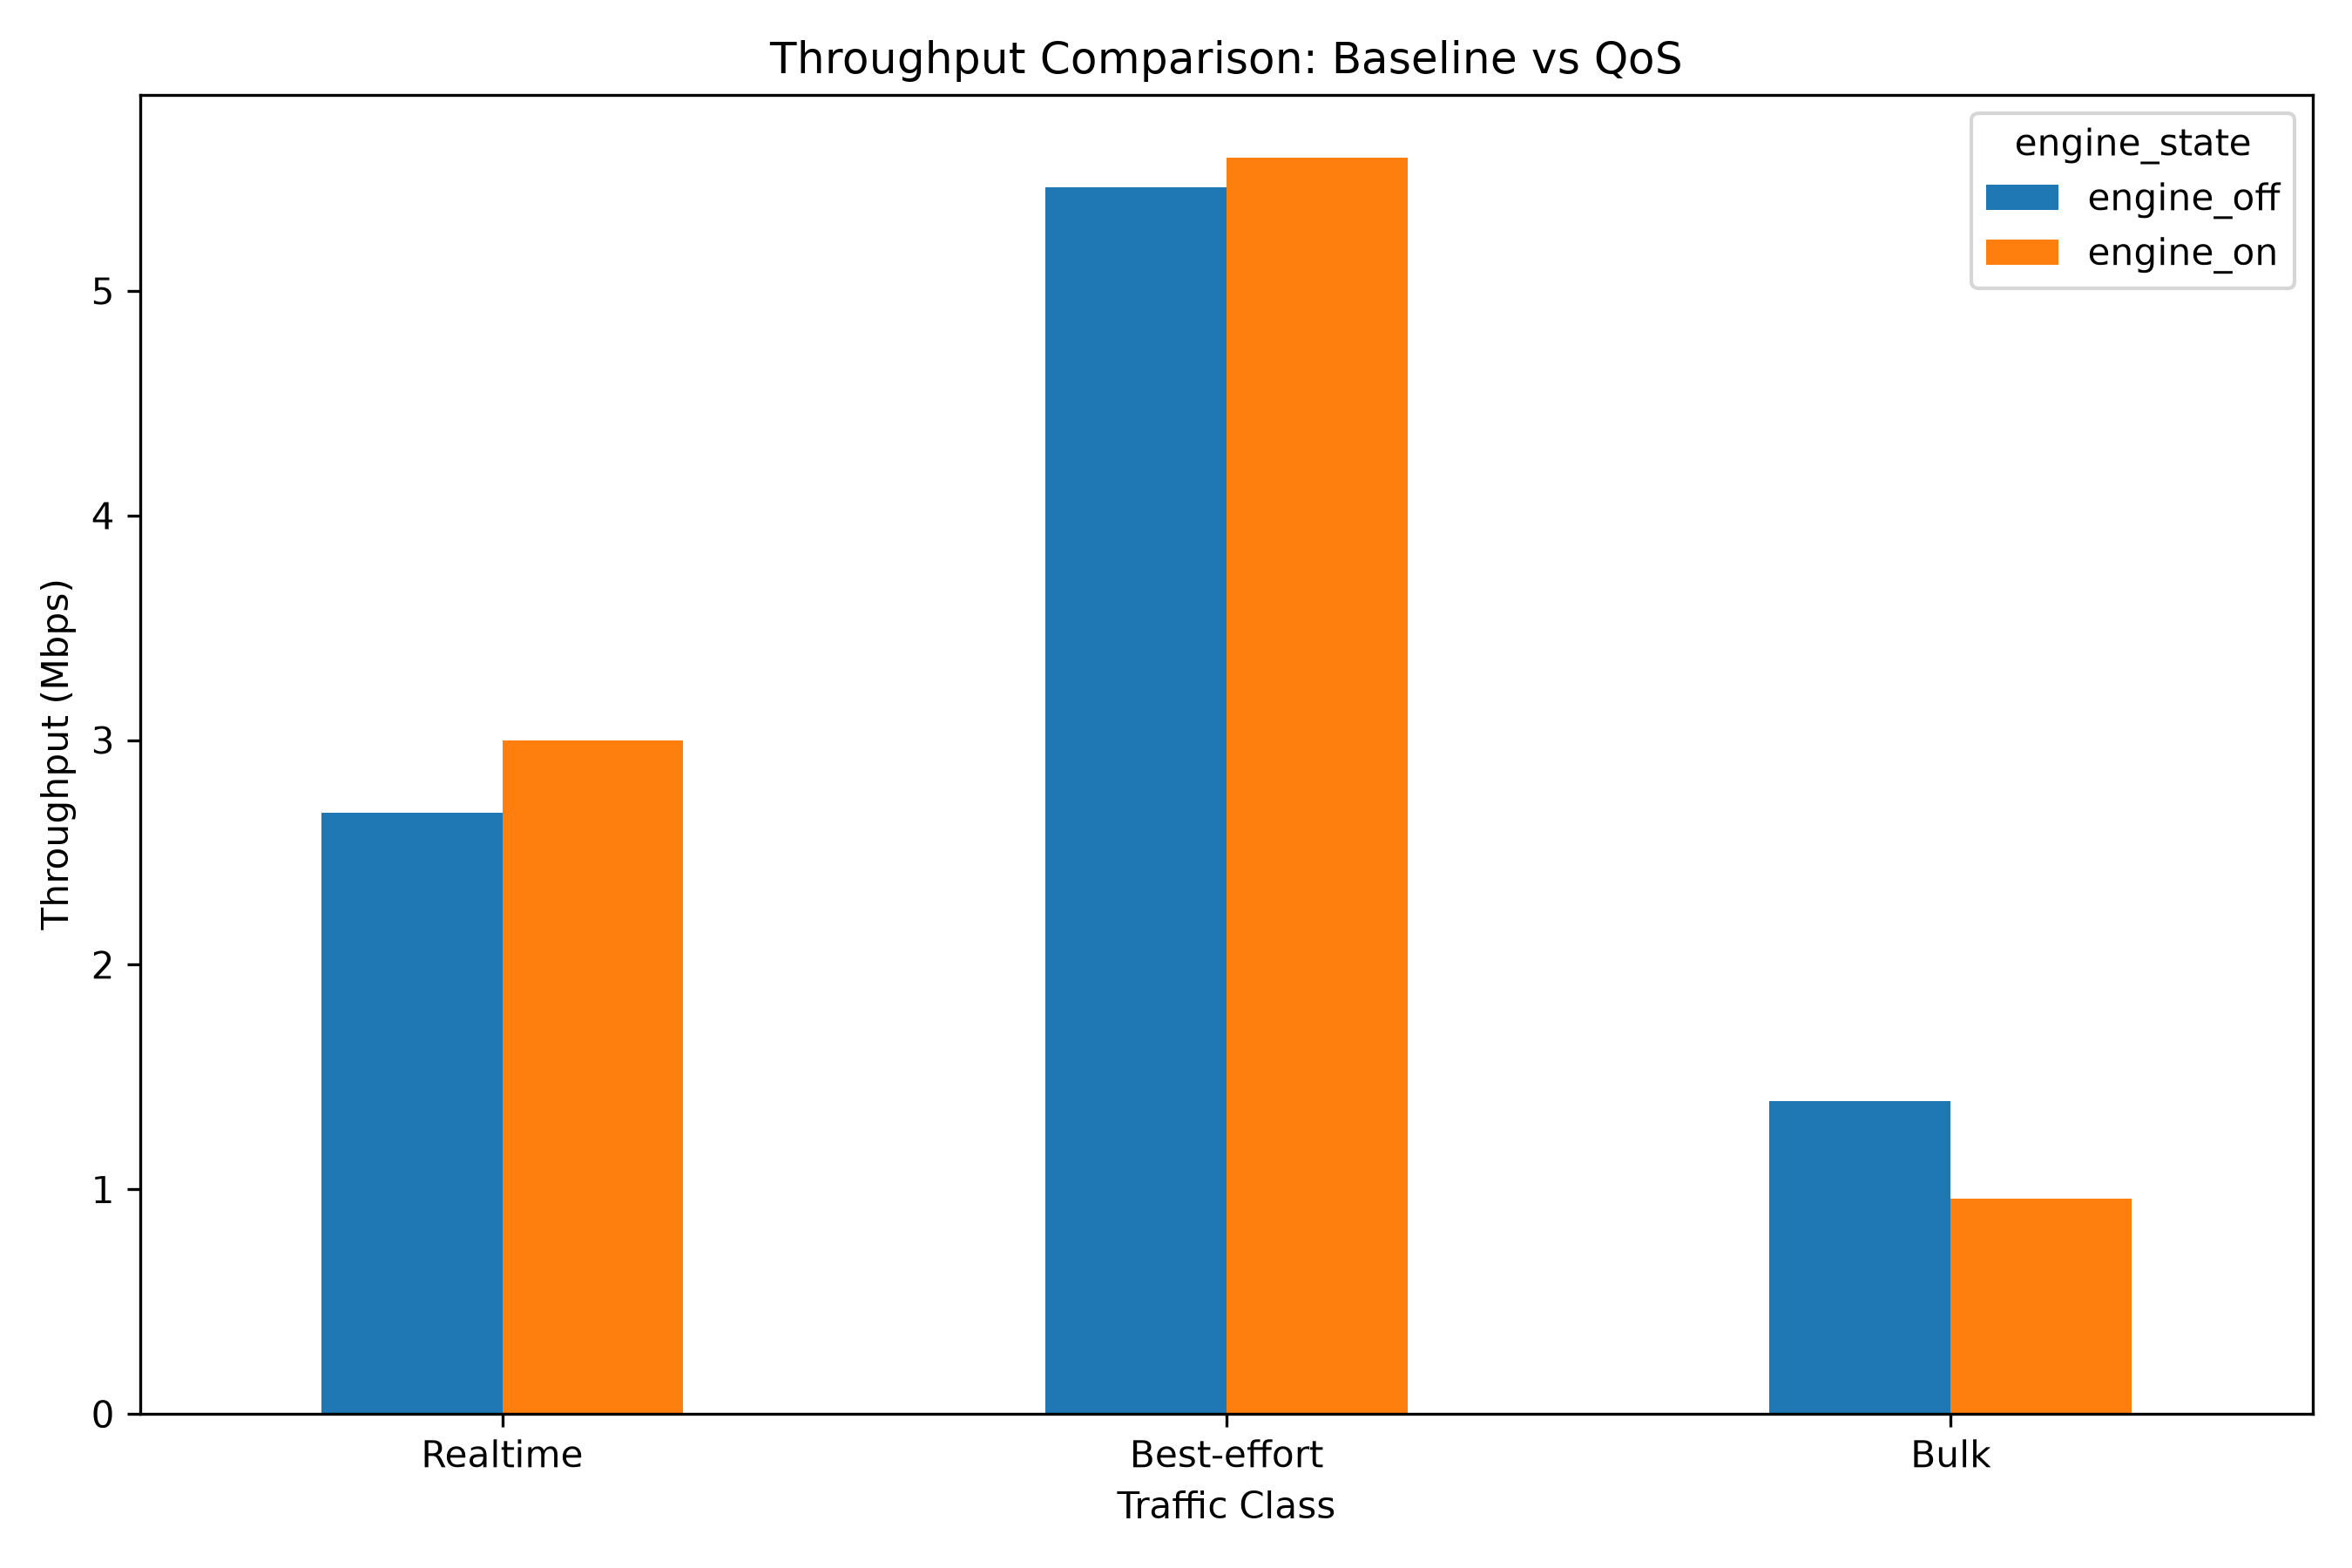
\includegraphics[width=\columnwidth]{results/throughput_comparison.png}
\caption{Throughput comparison between the baseline (Engine OFF) and QoS-enabled (Engine ON) configurations.}
\label{fig:throughput-comparison}
\end{figure}

\begin{figure}[t]
\centering
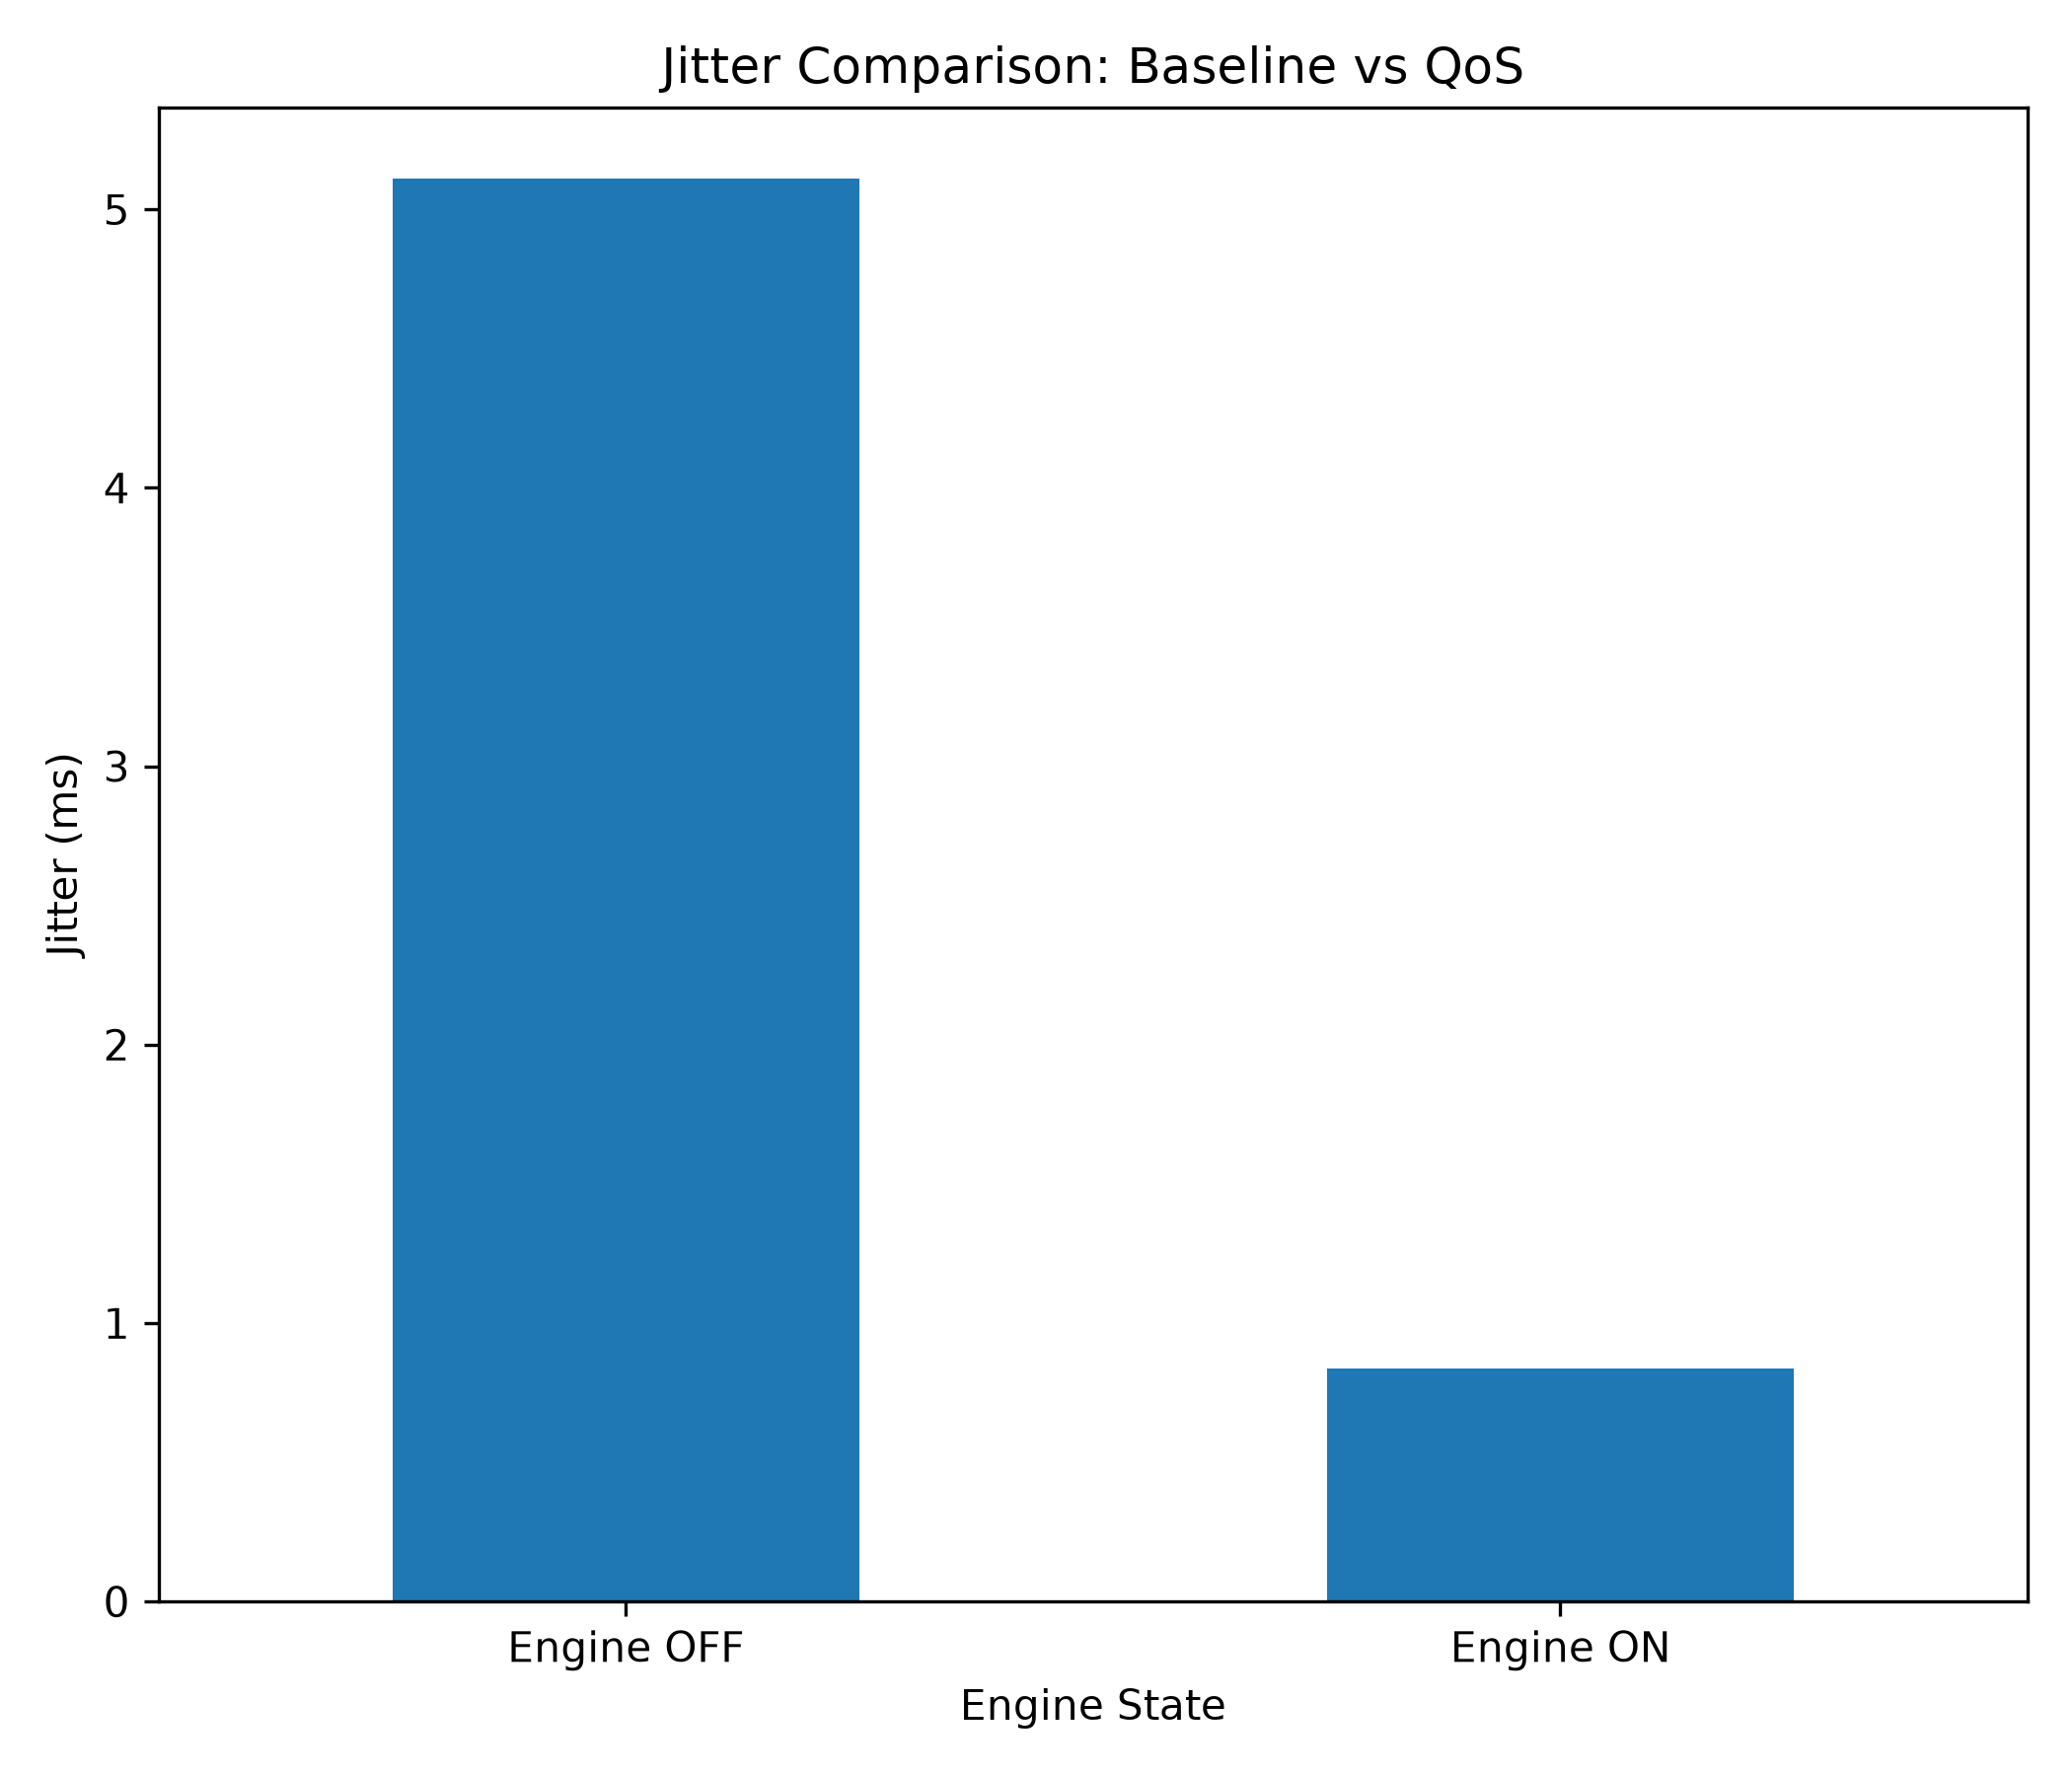
\includegraphics[width=\columnwidth]{results/jitter_comparison.png}
\caption{Realtime jitter comparison between the baseline (Engine OFF) and QoS-enabled (Engine ON) configurations.}
\label{fig:jitter-comparison}
\end{figure}


% =====================================================================
\section{Experimental Setup and Availability}
\label{sec:results-analysis}

\subsection{Experimental Setup}

All experiments were conducted on WSL2 Ubuntu 24.04 using Mininet
2.3.0, Open vSwitch 2.17, os-ken 2.1, and Python 3.11. The automated
experiment script (\texttt{automation/run\_all.sh}) runs three 15-second
trials for each engine state (OFF/ON), generating all three traffic
types simultaneously. OVS queue snapshots are captured per trial
(see \texttt{results/ovs\_snapshots/}) to verify rule installation.
Classifier training and QoS performance results are reported in
Section~\ref{sec:implementation}.

\subsection{GitHub Repository}

The complete source code, training data, experiment scripts, and
documentation are publicly available at:\\
\url{https://github.com/YazheneS/priority-based-network-trafficing}

The repository includes:
\begin{itemize}
  \item Mininet topology and OVS queue setup scripts
  \item Behavioral classifier with 1,701-sample training set
  \item Automated experiment runner and eval scripts
  \item Real-time monitoring dashboard (React + Node.js)
  \item Full Phase 1/2/3 verification documentation
\end{itemize}

% =====================================================================
\section{Conclusion}
\label{sec:conclusion}

We presented a fully automated SDN-based QoS system for campus
networks that classifies traffic by behavior (not port or IP) and
enforces differentiated service through a starvation-safe priority
engine. Four contributions from four independent papers—behavioral
classification (Serag et al.), fairness-aware bandwidth splitting
(Shahriar et al.), starvation prevention (Gorkemli et al.), and
motivation for behavioral over static approaches (Deo et al.)—are
integrated into a single working pipeline for the first time.

Experimental results on a Mininet-emulated campus segment show an
84\% reduction in real-time jitter (5.11~ms to 0.84~ms) and 97.6\%
classifier accuracy on 288 fresh held-out samples, with zero
realtime packet loss. The implementation is open-source and reproducible.

Future work includes scaling to multi-switch topologies, extending the
classifier to additional traffic categories, and evaluating the system
under higher-bandwidth links with more realistic campus traffic mixes.

% =====================================================================
\bibliographystyle{IEEEtran}
\bibliography{refs}

\end{document}
